\documentclass[conference]{IEEEtran}
\IEEEoverridecommandlockouts
% The preceding line is only needed to identify funding in the first footnote. If that is unneeded, please comment it out.
\usepackage{cite}

\usepackage{amsmath,amssymb,amsfonts,amsthm}
%\usepackage{algorithmic}
\usepackage{algorithm}
\usepackage{algpseudocode}
\usepackage{subfigure}
\usepackage{graphicx}
\usepackage{epstopdf}
\usepackage{textcomp}
\usepackage{multirow}
\usepackage{xcolor}
\newtheorem{definition}{Definition}
\newtheorem{theorem}{Theorem}
\newtheorem{lemma}{Lemma}
\renewcommand{\algorithmicrequire}{ \textbf{Input:}}
\renewcommand{\algorithmicensure}{ \textbf{Output:}}

\makeatletter
\newenvironment{breakablealgorithm}
  {% \begin{breakablealgorithm}
   \begin{center}
     \refstepcounter{algorithm}% New algorithm
     \hrule height.8pt depth0pt \kern2pt% \@fs@pre for \@fs@ruled
     \renewcommand{\caption}[2][\relax]{% Make a new \caption
       {\raggedright\textbf{\normalsize{Algorithm}~\thealgorithm} ##2\par}%
       \ifx\relax##1\relax % #1 is \relax
         \addcontentsline{loa}{algorithm}{\protect\numberline{\thealgorithm}##2}%
       \else % #1 is not \relax
         \addcontentsline{loa}{algorithm}{\protect\numberline{\thealgorithm}##1}%
       \fi
       \kern2pt\hrule\kern2pt
     }
  }{% \end{breakablealgorithm}
     \kern2pt\hrule\relax% \@fs@post for \@fs@ruled
   \end{center}
  }
\makeatother

\def\BibTeX{{\rm B\kern-.05em{\sc i\kern-.025em b}\kern-.08em
    T\kern-.1667em\lower.7ex\hbox{E}\kern-.125emX}}
\begin{document}

\title{The Communication Performance of BCDC Data Center Network\\
{\footnotesize \textsuperscript{}}
}

\author{\IEEEauthorblockN{Shuangxiang Kan, Jianxi Fan$^{*}$, Baolei Cheng}
\IEEEauthorblockA{School of Computer Science and Technology,\\ Soochow University \\
Suzhou, China \\
jxfan@suda.edu.cn}
\and
\IEEEauthorblockN{Xi Wang}
\IEEEauthorblockA{School of Software and Services Outsourcing,\\ Suzhou Institute of Industrial Technology \\
Suzhou, China \\
wangxi0414@suda.edu.cn}
}

\maketitle

\begin{abstract}
The BCDC network is a new server-centric data center network based on crossed cube. Its decentralized and recursively defined features solve the bandwidth bottleneck problem of the upper switch in the tree structure and make it more scalable. In addition, the degree of BCDC server is constant, which reduces connection cost and technical difficulty relative to DCell and BCube. In this paper, we study and analyze the data communication, fault tolerance, and node-disjoint paths of BCDC through practical experiments. The results show that BCDC is superior to DCell and Fat-Tree in data communication. Moreover, in terms of fault-tolerant routing and node-disjoint paths, the performance of BCDC is no worse than that of DCell and Fat-Tree. We also propose a one-to-one communication algorithm in BCDC under 1-restricted connectivity, analyze time complexity of algorithm, and give an upper bound of the conditional faulty diameter of BCDC under 1-restricted connectivity. The work in this paper provides an important basis for the design and application of the new data center network.\\
\end{abstract}

\textbf{\emph{Keywords-BCDC; data communication; fault tolerance; node-disjoint paths; data center network; 1-restricted connectivity}}

%\begin{IEEEkeywords}
%BCDC, data communication; fault tolerance; node-disjoint paths; data center network; 1-restricted connectivity
%\end{IEEEkeywords}

\section{Introduction}

The performance of the data center network largely determines the performance of cloud computing. Therefore, we can improve the performance of cloud computing by building a data center network with good performance. As the size and complexity of data center networks grows, so does the number of servers in data center networks. For example, Google had 450,000 servers in 2006, and by the end of 2010, its number of servers had reached more than 900,000. In a data center network with such a large number of servers, how to connect these servers to form a good performance data center network is a challenge to improve cloud computing performance. There are many factors that determine the performance of a data center network, communication performance and fault tolerance are significant aspects of them:\\
\textbf{Communication performance}: Many applications deployed on data center networks, such as web page retrieval, games, etc., have much more traffic between servers than traffic with external customers. These applications are all implemented through data communication between servers. Therefore, a good data center network should be able to support some typical data transmission methods, such as one-to-one, one-to-many, one-to-all, and all-to-all, etc.
On the other hand, improving data transmission bandwidth is also the goal of data center network design. \\
\textbf{Fault tolerance}: Due to the large number of switches and servers in the data center network, it is difficult to avoid the failure of switches,  servers, and links. Therefore, in the application of the data center network, it must be considered how to make the network work normally when some resources (servers, switches, or links) fail, that is, the data center network must consider fault tolerance.

Scalability and cost are also two important aspects of evaluating data center network. With the continuous expansion of data scale, good scalability and low cost will effectively promote the expansion of data center network and the processing of data.

In order to meet the above requirements, various data center networks have been proposed so far\cite{AlFaresM2008,GuoC2008,GuoC2009,XuM2019,NasirianS2019,XieP2019}. Such as traditional tree structure, Fat-Tree \cite{AlFaresM2008,LeisersonCE1985}, DCell\cite{GuoC2008,LvM2018}, and BCube\cite{GuoC2009}, etc. However, these factors are mutually influential and mutually restrictive. For example, although the Fat-Tree is simple in structure and easy to implement, its tree structure makes it weak in fault tolerance, uneven bandwidth distribution, insufficient scalability, and high cost. It cannot support one-to-many and many-to-many network communication well; The data center network represented by DCell has better routing performance and high scalability. However, when the switches become faulty, the length of the fault-tolerant path between servers will increase significantly.

A new data center network based on crossed cube was proposed in \cite{wang2018bcdc}, which is denoted by BCDC. An $n$-dimensional BCDC can be constructed recursively from two $(n-1)$-dimensional BCDCs. In an $n$-dimensional BCDC, each server has 2 ports connected to 2 switches, and each switch is equipped with $n$ ports connected to $n$ servers. Because each server is equipped with two ports, the reliability of BCDC will not be greatly affected even if one of the ports becomes faulty.

A lot of theoretical work has been done on BCDC network, so in this paper, we mainly focus on the experimental research of BCDC properties. This will provide an important basis for the deployment possibility of BCDC. The experiments in this paper mainly use the algorithm in \cite{wang2018bcdc} to verify the performance of BCDC's data communication, fault tolerance, and node-disjoint paths. So in order to better understand our experiments, we first introduce the algorithms to be used in our experiments. At the same time, we propose one-to-one communication algorithm in BCDC under 1-restricted connectivity, which shows that BCDC can communicate normally when the number of faulty nodes does not exceed $3n-5$ if any node has at least one fault-free neighbor in BCDC. Then we carry out corresponding experiments on data communication, fault tolerance and node-disjoint paths of $3$-dimensional BCDC. Besides, we also conducted comparison experiments on two other famous data center networks, DCell and Fat-Tree. The experimental results show that BCDC has superior data communication performance, and its performance in fault tolerance and node-disjoint paths is not inferior to DCell and Fat-Tree.

The organization of the paper is as follows, we will give the definition and construction method of BCDC in section \ref{structure}. Then in section \ref{algorithms}, we introduce the data communication, fault tolerance, and node-disjoint paths algorithms to be used in the experiments and present one-to-one communication algorithm in BCDC under 1-restricted connectivity. In section \ref{experiment}, experiments and analysis of the BCDC data communication, fault-tolerant routing, and node-disjoint paths are given. Section \ref{conclusion} concludes the paper.


\section{Physical and Logical Structure of BCDC}\label{structure}

We use the graph $G$ to represent a data center network. The switch can be considered as a transparent network device\cite{GuoC2008} in the data center network, so the node can be used to represent the server and the edge represents the link between servers in the data center network. We use $V(G)$ and $E(G)$ to represent the node set and edge set of the graph $G$, respectively. We use $N_G(u)$ to represent all nodes adjacent to node $v$. If $U \in V(G)$, then $N_G(U)=\bigcup_{u \in U}N_G{(u)}-U$. Let $u,v \in V(G)$, the distance between $u$ and $v$ in the graph $G$, denoted by $dist(G,u,v)$, is defined as the length of the shortest path between $u$ and $v$ in the graph $G$. The diameter of graph $G$, denoted by  $d(G)$, $=\max\{dist(G,u,v) \mid u,v \in V(G)\quad \mbox{and} \quad u \neq v\}$. Let $V^{'}\subseteq V(G)$, we use $G[V^{'}]$ to represent the subgraph in $G$ that are derived from the node subset $V^{'}$. $Connectivity$ is the minimum number of nodes that need to be deleted to make a connected graph $G$ become disconnected, denoted by $\kappa(G)$. However, the probability that all nodes adjacent to a node will fail at the same time is very small in reality. Therefore, in this paper, we propose the algorithm for two faulty-free nodes to communicate under the condition of 1-restricted connectivity. The $g$-$restricted$ $connectivity$, denoted by $\kappa_g(G)$, is a minimum set of faulty nodes $F$, after deleting $F$, $G$ will become an unconnected graph or a trivial graph, and the degree of each node is at least $g$.
%For more works on $g$-restricted connectivity, see \cite{LvMJ,LiX2018,LiXJ2019,LinL2018}.

A path $P=\langle x_0,x_1,\ldots,x_{n-1}\rangle$ of length $n-1$ is a finite non-empty sequence with different nodes such that $(x_i,x_{i+1}) \in E(G)$ for $0\leq i\leq n-2$. We also use $\langle x_0,\ldots,x_i,Q,x_j,\ldots,x_{n-1} \rangle$ to denote path $P$, where $Q$ is the subpath $\langle x_{i+1},x_{i+2},\ldots,x_{j-1}\rangle$. The reverse of path $P$ is $\langle x_{n-1},x_{n-2},\ldots,x_0\rangle$, denoted by $P^{-1}$. Moreover, $subpath(P, x_i,x_j)$ is used to represent a subpath of $P$ which starts at node $x_i$ and ends at node $x_j$. We also use $P[i]$ to denote node $x_i$ in $\langle x_0,x_1,\ldots,x_{n-1}\rangle$ and use $P[-2]$ and  $P[-1]$ to denote the penultimate and the last nodes in $P$, respectively.

As mentioned above, we intend to construct a data center network based on the $n$-dimensional crossed cube, denoted by $CQ_n$, which has better performance in many aspects than other networks. See \cite{DBLPEfe,Chang2000Edge,GuoJ2019} for the specific definition and properties of crossed cube.

BCDC is a data center network based on the crossed cube. We will deploy switches on the nodes of $CQ_n$ and servers on the edges of $CQ_n$. For the convenience of description, We do not distinguish between each switch and its address. The same is true for each server and its address.

The address of each switch is denoted by a $n$-bit binary string $x=x_{n-1}x_{n-2}\ldots x_0$. The address of each server is represented as an ordered pair $[x,y]$, where $x$ and $y$ are two $n$-bit binary strings $x=x_{n-1}x_{n-2}\ldots x_0$ and $y=y_{n-1}y_{n-2}\ldots y_0$. A server $[x,y]$ is connected to a switch $u$ if and only if $u\in \{x,y\}$ and $(x,y)\in E(CQ_n)$. Thus, we derive the original graph $A_n$ of the $n$-dimensional BCDC network.

Considering that the switch is transparent in the BCDC network, we can give the definition of the logical graph of the BCDC network as follows:



\begin{figure*}[htbp]
\centerline{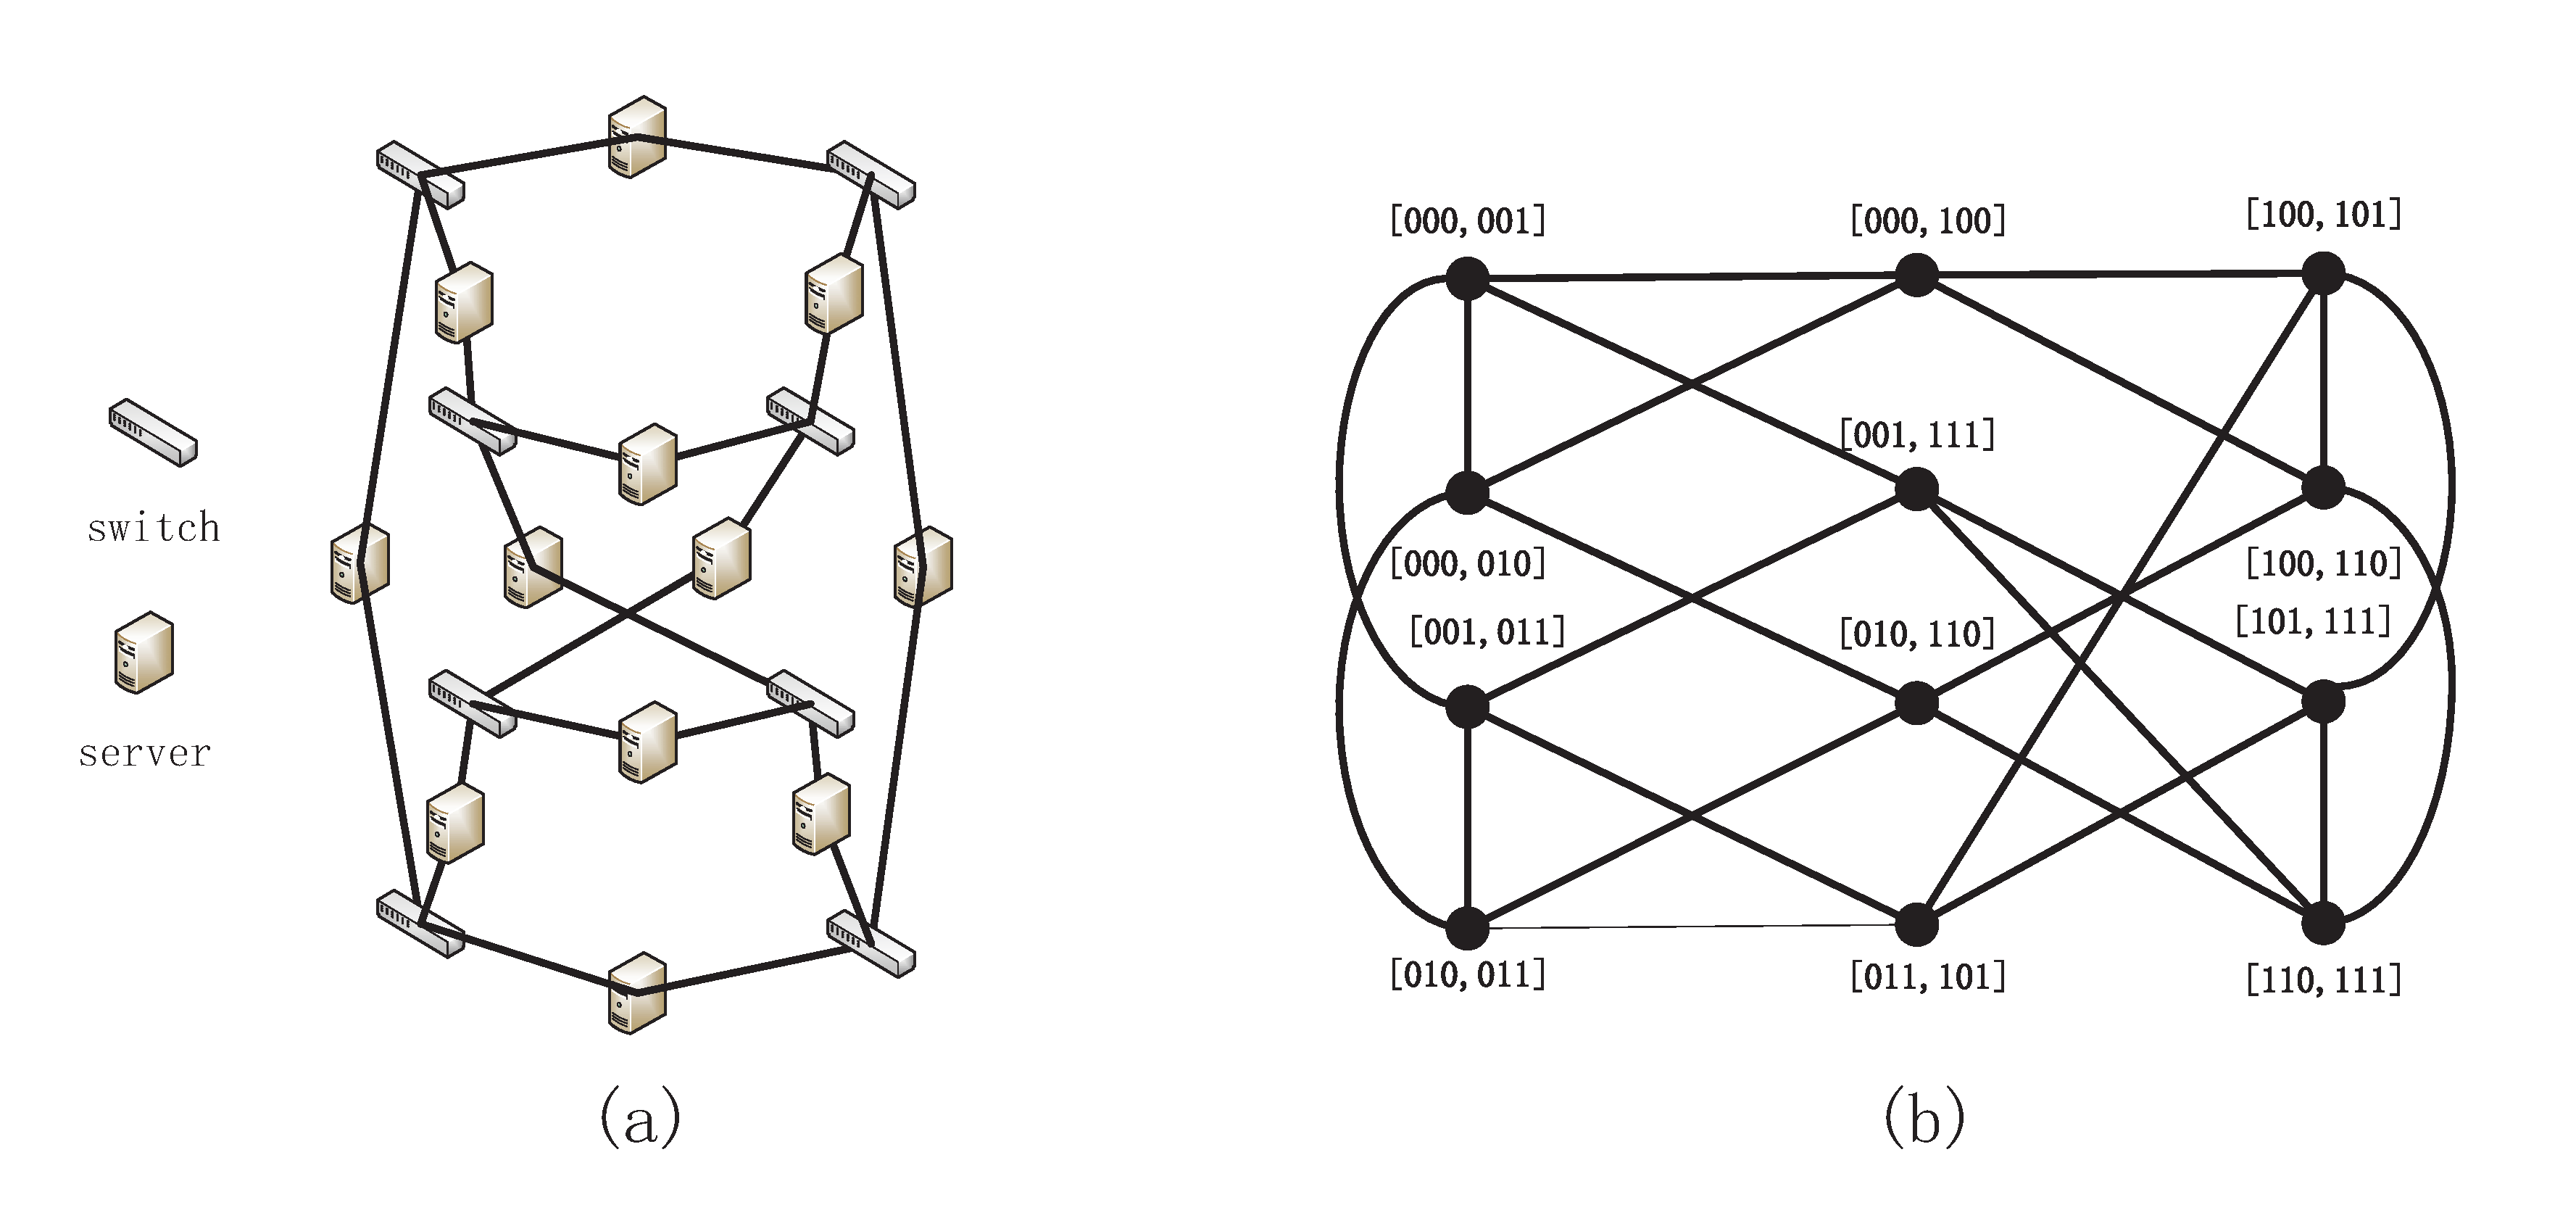
\includegraphics[scale=0.2]{A3B3.eps}}
\caption{(a)The original graph of 3-dimensional BCDC $A_3$,
(b)The logical graph of 3-dimensional BCDC $B_3$.}
\label{original-logical-bcdc3}
\end{figure*}

%\begin{figure*}[ht]
%\centering
%% Requires \usepackage{graphicx}
%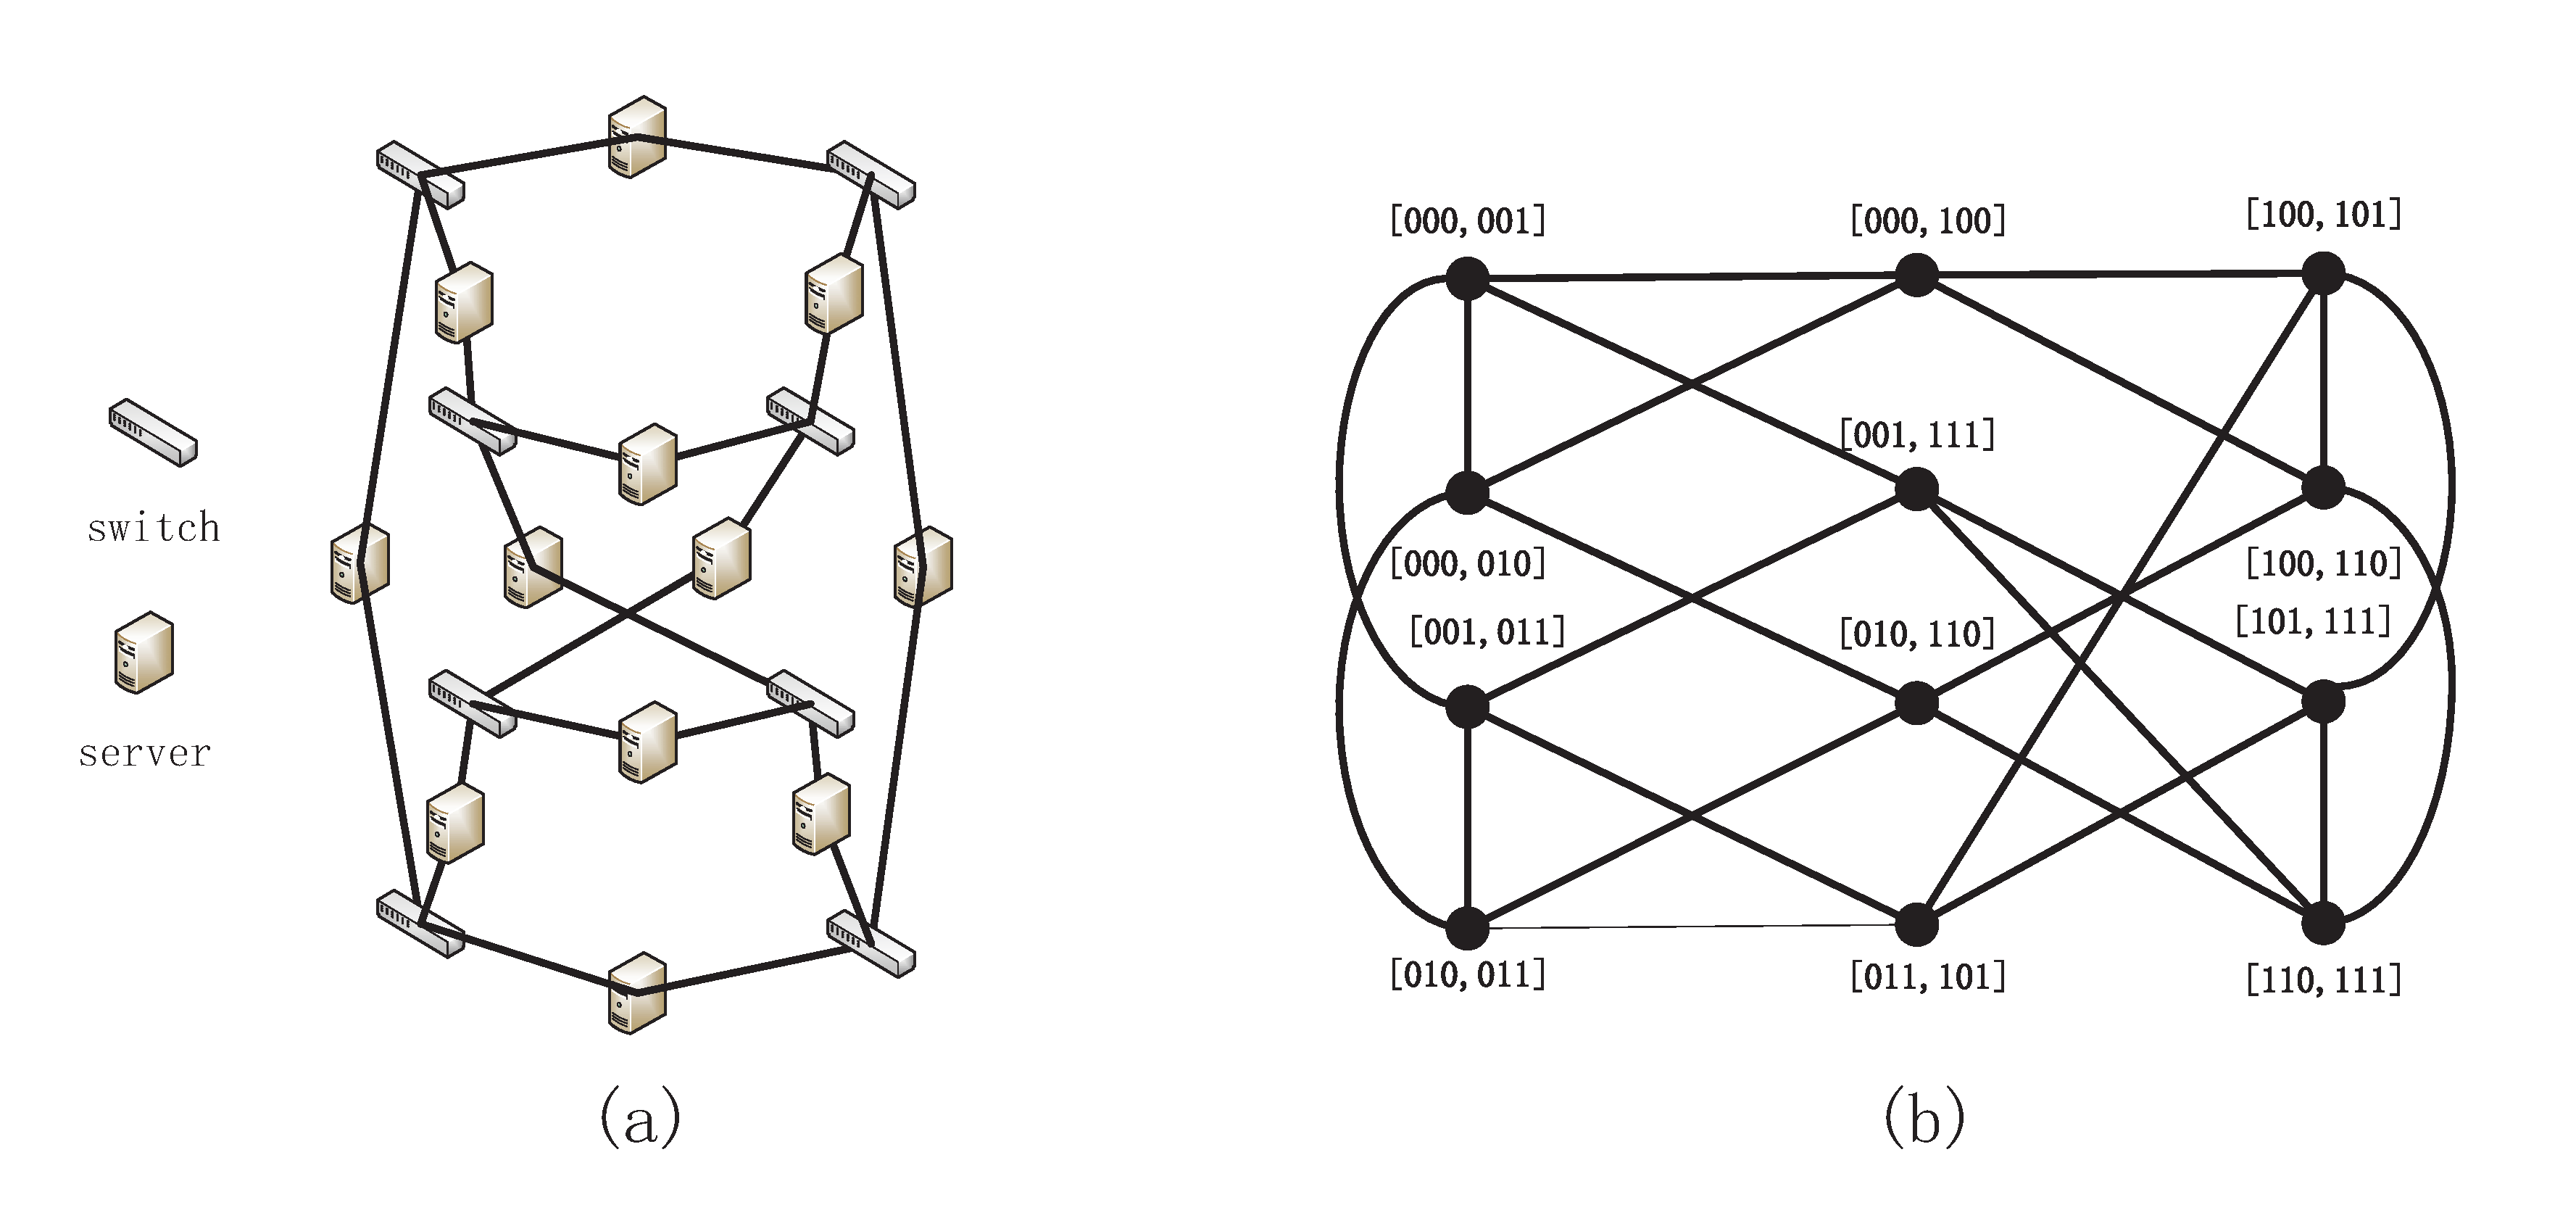
\includegraphics[scale=0.25]{A3B3.eps}\\
%\caption{(a)The original graph of 3-dimensional BCDC $A_3$,
%(b)The logical graph of 3-dimensional BCDC $B_3$}
%\label{original-logical-bcdc3}
%\end{figure*}


\begin{definition}
\label{Defi-BCDCn}
\cite{wang2018bcdc}
The $n$-dimensional BCDC network$,$
$B_n,$
is recursively defined as follows$.$
$B_2$ is a cycle with $\rm{4}$ nodes
$[00,01],$
$[00,10],$
$[01,11],$ and
$[10,11].$
For $n \geq 3,$
we use $B^0_{n-1}$ $($resp$.$ $B^1_{n-1}$$)$ to denote
the graph obtained by $B_{n-1}$ with changing each node $[x,y]$ of $B_{n-1}$ to $[0x,0y]$ $($resp$.$ $[1x,1y]$$).$
$B_n$ consists of $B^0_{n-1}$, $B^1_{n-1},$  and a node set
$S_n = \{ [a,b] | a \in V(CQ_{n - 1}^0),$ $b \in V(CQ_{n - 1}^1),$ and $(a,b) \in E(C{Q_n})\}$
according to the following rules$.$
For nodes  $u = [a,b] \in V(B_{n - 1}^0),$ $v = [c,d] \in S_n,$ and $w = [e,f] \in V(B_{n - 1}^1)$$:$

$1)$  $(u,v) \in E(B_n)$ if and only if $a = c$ or $b = c.$

$2)$  $(v,w) \in E(B_n)$ if and only if $e = d$ or $f = d.$
\end{definition}


The original and logical graphs of the $3$-dimensional BCDC network are shown in Fig. \ref{original-logical-bcdc3}.

Then, we give several properties of BCDC.

\begin{theorem}
\label{kappabn}
\cite{wang2018bcdc}
$\kappa(B_n) = 2n-2.$
\end{theorem}

\begin{lemma}
\label{diameterBn}
\cite{wang2018bcdc}
The diameter of $B_n$ is $\lceil\frac{n+1}{2}\rceil+1$.
\end{lemma}

\begin{lemma}
\label{restrictedConnectivity}
\cite{LvMJ}
For any integer $n \geq 3$, $\kappa_1(B_n)=3n-4.$
\end{lemma}

\section{Data Communication, Fault-tolerant Routing, and Node-Disjoint Paths
Algorithms of BCDC}\label{algorithms}

\subsection{Fault-Free Routing in BCDC}\label{dataCommunication}
In this section, we introduce efficient data communication algorithms on BCDC, including one-to-one, one-to-many, one-to-all, and all-to-all algorithms.
\subsubsection{One-to-One Routing}

Efe\cite{DBLPEfe} proposed an algorithm for finding the shortest path between any two nodes in $CO_2$ with time complexity of $O(n^2)$.
Chang et al.\cite{Chang2000Edge} improved Efe's algorithm and proposed an algorithm $CSH(CQ_n, u, v)$ with time complexity of $O(n)$. Moreover, they provided a $\rho(u,v)$ function for quickly calculating the distance between any two nodes on $CQ_n$ and $\rho(u,v)=dist(CQ_n,u,v)$. In \cite{wang2018bcdc}, Wang et al. proposed a algorithm $BRouting$ based on the $CSH(CQ_n, u, v)$ algorithm to find the shortest path of any two nodes in BCDC with a time complexity of $O(n)$. Since any two nodes $u, v$ in BCDC are represented by four nodes $[u_1, u_2]$ and $[v_1, v_2]$ in $CQ_n$, $BRouting$ algorithm uses the shortest path in $CSH(CQ_n, u_1, v_1)$, $CSH(CQ_n, u_1, v_2)$, $CSH(CQ_n, u_2, v_1)$,  and $CSH(CQ_n, u_2, v_2)$ to construct the shortest path between $u$ and $v$. The length of routing path between $u$ and $v$ constructed by Algorithm $BRouting$ is no more than $\lceil\frac{n+1}{2}\rceil+1$. The BCDC's one-to-one data communication in our later experiments will be based on the $BRouting$ algorithm.


\subsubsection{One-to-Many Routing}

Wang et al.\cite{wang2018bcdc} proposed a algorithm $BMulticast$ with time complexity $O(n|T|^2)$ to realize one to many communication in BCDC, where $T$ is the set of destination nodes. The $BMulticast$ algorithm constructs $|T|$ paths from the source node to the destination nodes by calling BRouting algorithm $|T|$ times, and merges the common nodes and paths to construct a multicast tree. The height of the multicast tree constructed
by algorithm $BMulticast$ is no more than $\lceil \frac{n+1}{2} \rceil +1$.



\subsubsection{One-to-All(Broadcast) and All-to-All Routing}
%However, a multicast tree constructed in $BMulticast$ has a problem, that is, if a common node of the multicast tree fails, all leaf(destination) nodes in the subtree rooted at the faulty node will not be able to receive data sent by the source node . In addition, merging common nodes and paths multiple times also consumes certain resources. Therefore, in the experiment, we will not use $BMulticast$ algorithm to construct a broadcast tree to implement the broadcast communication of BCDC. We will propose a broadcast algorithm similar to the breadth-first search algorithm, which is called $BBroadcast$, to implement BCDC's broadcast communication.
%
%\begin{breakablealgorithm}
%\label{BBroadcast}
%    \caption{\texttt{BBroadcast}}
%\footnotesize
%    \begin{algorithmic}[1]
%    \Require an $n$-dimensional BCDC, $B_n$; $s \in V(B_n)$;
%    %$D \subset V(B_n)$ and $\{s\} \cap D  = \emptyset$.
%    \Ensure  a multicast tree $MT$ rooted at node $s$ to nodes in a node set  $D$ on $B_n$.
%    \Function{\texttt{BBroadcast}}{$B_n,s$}%
%    %\State $V(MT) \gets \{s\}$;
%%    \State $E(MT) \gets \emptyset$;
%    \For{each $u \in N_G(s)$}
%        \If{If $u$ has not received the data packet}
%            \State Mark $u$ has received the packet;
%        \EndIf
%        \State $D=D \setminus \{u\}$;
%        \State \texttt{BBroadcast}($B_n,v$)
%
%
%    \EndFor
%    %\State\Return $MT$;
%    \EndFunction
%  \end{algorithmic}
%\end{breakablealgorithm}

For the broadcasting algorithm in BCDC, we will use $BMulticast$ algorithm to implement it, using one of the nodes in BCDC as the source node and the remaining nodes as destination nodes, and using $BMulticast$ to construct a broadcast tree to implement data transmission. Since the diameter of $B_n$ is $\lceil\frac{n+1}{2}\rceil+1$, then the height of broadcast tree constructed by Algorithm $BMulticast$ is no more than $\lceil\frac{n+1}{2}\rceil+1$. For full exchange communication, we also use the $BMulticast$ algorithm to construct a broadcast tree rooted at each node in $B_n$. Then, each node in $B_n$ performs data transmission along the broadcast tree rooted at it, thereby implementing all-to-all communication.

%
%In the broadcast of a data center network, we can construct a spanning tree from the source node to all other nodes to transmit data packets. However, the spanning tree of a data center network is not fault tolerant. If a node of the spanning tree becomes faulty, the subtree rooted at this node will not receive the data sent by the source node.
%
%% ����㲥�㷨������û�ģ�Ҫ��һ��
%Therefore, in order to solve the shortcoming of low fault-tolerance of the spanning tree, we propose a simply broadcast scheme in BCDC, called $BBroadcast$: the source node sends a data packet to its $2n-2$ neighbor nodes. When one of these nodes receives the data packet, it first checks if this data packet has been received before. This data packet will be discarded if it has been received before, otherwise, the packet is received and then sent to all its neighbor nodes, and so on. The $BBroadcast$ scheme is a simple and good fault-tolerant algorithm that ensures that packets can reach every node in the BCDC network when the BCDC network is connected. Since the diameter of $B_n$ is $\frac{n+1}{2}+1$, then the height of broadcast tree constructed by Algorithm OTMRouting is no more than $\frac{n+1}{2}+1$.
%
%For all-to-all communication, we can use $BBroadcast$ scheme to construct a broadcast tree rooted at each node in $B_n$. Then, each node in $B_n$ performs data transmission along the broadcast tree rooted at it, thereby implementing all-to-all communication.

\subsection{Fault-Tolerant Routing and One-to-One Communication under 1-Restricted Connectivity in BCDC}\label{restrictedConnectivity}
Assume that there is a faulty nodes set $F$ in BCDC network, then how to find a shortest fault-free path between any two fault-free nodes in a short period of time is an important issue in BCDC that need to be addressed.

Wang et al.\cite{wang2018bcdc} proposed an algorithm $BFRouting$ for finding a one-to-one fault-free path in BCDC when $|F|\leq 2n-3$. This is also the algorithm we used in our experiments. However, we also observe that \cite{wang2018bcdc} has the premise that it assumes that all adjacent nodes of a node may fail at the same time, but this has a small probability of appearing in the actual running environment of the data center network. Therefore, in this paper, we propose a one-to-one communication algorithm $ BRFTRouting$ for BCDC under 1-restricted
connectivity. There are many similarities between the $BFRouting$ algorithm and the $ BRFTRouting$ algorithm. The main difference between the two algorithms is the number of faulty nodes and the limitation of node fault conditions. The number of faulty nodes of 1-restricted connectivity is $|F|\leq 3n-5$ and each node has at least one fault-free neighbor.

\begin{theorem}\label{grestricted}
\cite{LvMJ}
Let $u,v \in V(B_n)$ and $(u,v) \in E(B_n)$, then $N_{B_n}(\{u,v\})=3n-4$.
\end{theorem}

%\begin{lemma}
%\label{mappingPath}
%For any integer $n \geq 3,$  any faulty node set $F \subset V(B_n)$ with $|F| \leq 3n-5,$
%and any $u \in V(B_{n-1}^{i}) - F$ with $i \in \{0,1\},$
%there exists at least one fault-free path $P = \langle\alpha_0 = u, \alpha_1, \ldots, \alpha_l\rangle$ of length $l$ with $2 \leq l \leq 4,$
%from $u$ into $B_{n-1}^{{1-i}},$  such that
%$\alpha_0, \alpha_1, \ldots, \alpha_{l-2} \in V(B_{n-1}^{i}),$
%$\alpha_{l-1} \in S_n,$  and
%$\alpha_l \in V(B_{n-1}^{{\bar{i}}}).$
%\end{lemma}
%
%\begin{proof}
%Without loss of generality, suppose that $i = 0$. Let $(u,v) \in E(B_n)$, then we have the following two cases:
%
%\textbf{Case 1:} $v \in V(B_n^{0})$. Let $\alpha_1, \alpha_2, \alpha_3, \beta_4, \beta_5, \ldots$, $\beta_{2n-1}$, $\gamma_{2n}, \gamma_{2n+1}, \ldots$, and $\gamma_{3n-4}$ be all the $3n-4$ neighbors of $u$ and $v$, with
%$\alpha_1, \alpha_2, \alpha_3 \in S_n$, $(u,\beta_i) \in E(B^0_n)$ for $4\leq i \leq 2n-1$, and $(v,\gamma_i) \in E(B^0_n)$ for $2n \leq i \leq 3n-4$.
%Choose $3n-7$ nodes $\alpha_4, \alpha_5, \ldots, \alpha_{3n-4}$
%in $S_n$ such that $(\beta_i,\alpha_i) \in E(B_n)$ for $4 \leq i \leq 2n-1$ and $(\gamma_i,\alpha_i) \in E(B_n)$ for $2n \leq i \leq 3n-4$  with
%$|\{\alpha_1, \alpha_2, \ldots, \alpha_{3n-4}\}|= 3n-4$.
%Then, choose
%$3n-4$ nodes $\eta_1, \eta_2, \ldots, \eta_{3n-4}$
%in $B_{n-1}^{{1}}$
%such that
%$(\alpha_i,\eta_i) \in E(B_n)$ for $1 \leq i \leq 3n-4$ with
%$|\{\eta_1, \eta_2, \ldots, \eta_{3n-4}\}| = 3n-4$.
%
%
%As a sequence, we construct $3n-4$ disjoint paths from $B_{n-1}^{{0}}$
%into $B_{n-1}^{{1}}$ as follows:
%\begin{align*}
%P_1     = &   \langle u, \alpha_1, \eta_1\rangle,  \\
%P_2     = &   \langle u, \alpha_2, \eta_2\rangle,  \\
%P_3     = &   \langle u, v, \alpha_3, \gamma_3\rangle,  \\
%P_{4}   = &   \langle u, \beta_4, \alpha_4, \eta_4\rangle, \\
%P_{5}   = &   \langle u, \beta_5, \alpha_5, \eta_5\rangle, \\
%\vdots &   \\
%P_{2n-3}= &   \langle u, \beta_{2n-1}, \alpha_{2n-1}, \eta_{2n-1}\rangle, \\
%P_{2n-2}= &   \langle u, v, \gamma_{2n}, \alpha_{2n}, \eta_{2n}\rangle, \\
%P_{2n-1}= &   \langle u, v, \gamma_{2n+1}, \alpha_{2n+1}, \eta_{2n+1}\rangle, \\
%\vdots &   \\
%P_{3n-5}= &   \langle u, v, \gamma_{3n-5}, \alpha_{3n-5}, \eta_{3n-5}\rangle, \textrm{ and}, \\
%P_{3n-4}= &   \langle u, v, \gamma_{3n-4}, \alpha_{3n-4}, \eta_{3n-4}\rangle.
%\end{align*}
%
%\textbf{Case 2:} $v \in S_n$. Let $\alpha_2, \beta_3, \beta_4, \ldots$, $\beta_{2n-3}$, $\gamma_{2n-2}, \ldots$, and $\gamma_{3n-4}$ be $3n-5$ neighbors of $u$ and $v$, with
%$\alpha_2 \in S_n$,$\gamma_i \in B^1_n$ for $2n-2 \leq i \leq 3n-4$, $(u,\beta_i) \in E(B^0_n)$ for $3 \leq i \leq 2n-3$, and $(v,\gamma_i) \in E(B_n)$ for $2n-2 \leq i \leq 3n-4$.
%Choose $2n-5$ nodes $\alpha_3, \alpha_4, \ldots, \alpha_{2n-3}$
%in $S_n$ such that $(\beta_i,\alpha_i) \in E(B_n)$ for $3 \leq i \leq 2n-3$.
%Then, choose
%$2n-3$ nodes $\eta_1, \eta_2, \ldots, \eta_{2n-3}$
%in $B_{n-1}^{{1}}$
%such that
%$(v,\eta_1) \in E(B_n)$ and $(\alpha_i,\eta_i) \in E(B_n)$ for $2 \leq i \leq 2n-3$.
%
%
%As a sequence, we construct $3n-4$ disjoint paths from $B_{n-1}^{{0}}$
%into $B_{n-1}^{{1}}$ as follows:
%\begin{align*}
%P_1     = &   \langle u, v, \eta_1\rangle,  \\
%P_2     = &   \langle u, \alpha_2, \eta_2\rangle,  \\
%P_{4}   = &   \langle u, \beta_3, \alpha_3, \eta_3\rangle, \\
%P_{5}   = &   \langle u, \beta_4, \alpha_4, \eta_4\rangle, \\
%\vdots &   \\
%P_{2n-3}= &   \langle u, \beta_{2n-3}, \alpha_{2n-3}, \eta_{2n-3}\rangle, \\
%P_{2n-2}= &   \langle u, v, \gamma_{2n-2}\rangle, \\
%P_{2n-1}= &   \langle u, v, \gamma_{2n}\rangle, \\
%\vdots &   \\
%P_{3n-5}= &   \langle u, v, \gamma_{3n-5}\rangle, \textrm{ and}, \\
%P_{3n-4}= &   \langle u, v, \gamma_{3n-4}\rangle.
%\end{align*}
%
%Since $|F| \leq 3n-5 < 3n-4$,
%there exists at least one fault-free path $P_j$ among the $3n-4$
%paths $P_1, P_2, \ldots, P_{3n-4}$,
%where $1 \leq j \leq 3n-4$.
%\end{proof}

Given a fault-free node $u$ of $B_n$, three subgraphs $S_1$, $S_2$, and $S_3$ of $B_n$ and a faulty node set $F$ with $|F|\leq 3n-5$, we give an algorithm, named by $BFinding$, to construct a fault-free path from $u$ to subgraph $S_3$. Since
the time complexity of finding a fault-free neighbor of $u$ in $B_n$ is $O(n)$, we can easily get the time complexity of $BFinding$ is $O(n^3)$.
%$BFinding$ includes two functions $BFinding1$ and $BFinding2$. In function $BFinding1$, according to definition \ref{Defi-BCDCn}, the time complexity of finding a fault-free neighbor of $u$ in subgraph $S_3$ is $O(n)$. In lines $9\sim13$ of function $BFinding2$, the number of operations required to find a fault-free path $(u, v, y)$ from node $u$ to subgraph $S_3$ is $O(n)$, where $u \in S_1$, $v\in S_2$, and $y\in S_3$. If there is no fault-free neighbor of $u$ in $S_2$, we will choose at most two intermediate fault-free nodes in $S_1$, then find the path that meets the requirement through intermediate nodes.
%Thus, in lines $14\sim20$ of function $BFinding2$, it  take $O(n^2$) time to construct a fault-free path $(u, x, v, y)$ from node $u$ to subgraph $S_3$, where $u,x \in S_1$, $v\in S_2$, and $y\in S_3$. Similarly, lines $21\sim29$ take $O(n^3$) time to construct a fault-free path $(u, x, v, w, y)$ from node $u$ to subgraph $S_3$, where $u,x,v \in S_1$, $w\in S_2$, and $y\in S_3$.  Therefore, the time complexity of $BFinding2$ is $O(n^3)$.

\begin{breakablealgorithm}
\footnotesize
\label{BFinding}
\caption{\texttt{{BFinding}}}
\begin{algorithmic}[1]
    \Require a fault-free node $u \in V(B_n)$, three subgraphs $S_1, S_2, S_3$ in $ B_n$,
    and  a faulty node set $F \subset V(B_n)$ with $|F|\leq 3n-5$, which does not contain all neighboring nodes of any node.
    \Ensure  a fault-free path from $u$ to $S_3$.
   \Function{\texttt{BFinding1}}{$u,S_3,F$}
   \For{$v \in N_{S_3}(u)$}
        \If{$v \notin F$}
            \State \Return($u,v$);
        \EndIf
   \EndFor
   \EndFunction


   \Function{\texttt{BFinding2}}{$u, S_1, S_2, S_3, F$}
   \For{$v \in N_{S_2-F}(u)$}
        \If{$N_{S_3}(v) \not\subseteq F$}
            \State \Return($u,\texttt{BFinding1}(v,S_3,F)$);
        \EndIf
   \EndFor
   \For{$x \in N_{S_1-F}(u)$}
        \For{$v \in N_{S_2-F}(x)$}
            \If{$N_{S_3}(v) \not\subseteq F$}
                \State \Return($u,x,\texttt{BFinding1}(v,S_3,F)$);
            \EndIf
        \EndFor
   \EndFor
   \For{$x \in N_{S_1-F}(u)$}
        \For{$v \in N_{S_1-F}(x)$}
            \For{$w \in N_{S_2-F}(v)$}
                \If{$N_{S_3}(w) \not\subseteq F$}
                    \State \Return($u,x,v,\texttt{BFinding1}(w,S_3,F)$);
                \EndIf
            \EndFor
        \EndFor
   \EndFor
   \EndFunction
  \end{algorithmic}
\end{breakablealgorithm}

%Then we give another sub-algorithm $BMerging$. Given a subgraph $G$ in $B_n$, a faulty node set $F$ in $B_n$, two fault-free nodes $u, v$, and two paths $P_1$ and $P_2$ obtained by algorithm $BFinding$, where $P_1[0]$=$u$, $P_2[0]$=$v$. We constructed a fault-free path from $u$ to $v$ in $B_n-F$ by algorithm $BMerging$. Because the algorithm $BMerging$ and the algorithm $BFTRouting$ call each other, that is, $BFTRouting$ is called in lines 5, 11, and 18 of the algorithm $BMerging$, and $BMerging$ is called in lines 24, 29, 32, 35, 38, 42, 45, and 49 of the algorithm $BFTRouting$, here we only analyze the time complexity of the part of the algorithm $BMerging$ that does not involve calling $BFTRouting$. The time complexity of the other parts will be analyzed after the algorithm $BFTRouting$ is given. In lines $2\sim4$ and $8\sim10$, it takes constant time to construct a fault-free path from $u$ to $v$ directly in $P_1$ or $P_2$. In lines $14\sim17$, it takes $O(n^2)$ time to find a node $x\in V(P_1)\cup V(P_2)$, which is the first common node of paths $P_1$ and $P_2$ and $O(1)$ time to connect the two subpaths of $P_1$ and $P_2$ together.
%
%
%\begin{breakablealgorithm}
%\footnotesize
%\label{BMerging}
%\caption{\texttt{{BMerging}}}
%\begin{algorithmic}[1]
%    \Require A subgraph $G$ of $B_n$, a fault node set $F$ of $B_n$, two fault-free node $u, v$, and two paths $P_1, P_2$, where $P_1[0]=u, P_2[0]=v$.
%    \Ensure  a fault-free path from $u$ to $v$ in $B_n - F$.
%
%    \Function{\texttt{BMerging1}}{$G, F, u, v, P_2$}
%    \If{$u \in V(P_2)$}
%        \State \Return $\texttt{Path}(P_2, u, v)$;
%    \EndIf
%    \State \Return (\texttt{BFTRouting}($G, F, u, P_2[-1])$, $P_2^{-1}$);
%    \EndFunction
%
%    \Function{\texttt{BMerging2}}{$G, F, u, v, P_1$}
%    \If{$v \in V(P_1)$}
%        \State \Return \texttt{Path}$(P_1, u, v)$;
%    \EndIf
%    \State \Return ($P_1$, \texttt{BFTRouting}($G, F, P_1[-1], v)$);
%    \EndFunction
%
%    \Function{\texttt{BMerging3}}{$G,F,u,v,P_1,P_2$}
%    \If{$V(P_1) \cap V(P_2) \neq \emptyset$}
%        \State Find a node $x\in V(P_1)\cup V(P_2)$, which is the first common node of paths $P_1$ and $P_2$;
%        \State \Return $(\texttt{Path}(P_1, u, x), \texttt{Path}(P_2^{-1}, x, v)$);
%    \EndIf
%    \State $S \gets \texttt{BFTRouting}(G, F, P_1[-1], P_2[-1])$;
%    \State \Return ($P_1$, $S$, $P_2^{-1}$);
%    \EndFunction
%  \end{algorithmic}
%\end{breakablealgorithm}

In the following $BRFTRouting$ algorithm, we will call $BFinding$ algorithm and  $BFRouting$ algorithm in \cite{wang2018bcdc} to construct
a fault-free path from $u$ to $v$ in $B_n-F$. In line 9 of the algorithm $BFTRouting$, we use $BFS$ to represent breadth-first search.


\begin{breakablealgorithm}
\label{BFTRouting}
\caption{\texttt{BRFTRouting}}
\footnotesize
    \begin{algorithmic}[1]
    \Require an $n$-dimensional BCDC, $B_n$,
    a faulty node set $F\subset V(B_{n})$ with $|F|\leq 3n-5$, which does not contain all neighboring nodes of any node
    and two fault-free node $u,v$.
    \Ensure  a fault-free path from node $u$ to $v$ in $B_n - F$.
    \Function{\texttt{BRFTRouting}}{$B_n,F,u,v$}%
%    \If{$u = v$}  \ \Return ($u$);
    \If{$(u,v)\in E(B_n)$}
        \State \Return ($u,v$);
    \ElsIf{$n = 2$}
        \State \Return (A fault-free path from $u$ to $v$ in $B_n - F$);
    \ElsIf{$|F| = 0 $}
        \State \Return \texttt{BRouting}$(B_{n},u,v)$;
    \ElsIf{$|F| \geq 3n-4$}
         \State \Return \texttt{BFS}($B_n-F,u,v$);
    \EndIf
    \State $F_{0}\gets F \cap V(B^{0}_{n-1})$;
    \State $F_{1}\gets F \cap V(B^{1}_{n-1})$;
    \State $F_{2}\gets F \cap  S_{n}$;
    \State $m \gets $min$\{|F_{0}|,|F_{1}|\}$;
    \For{$i \in \{0,1\}$}
        \State $B_0 \gets B^{i}_{n-1}$;
        \State $B_1 \gets B^{\bar{i}}_{n-1}$;
        \State $B_2 \gets B_n[S_{n}]$;
        \If{$u,v \in V(B_0)$ \textbf{and} $|F_{i}| = m$}
            \State \Return \texttt{BFRouting}($B_0, F_{i}, u, v$);
        \ElsIf{$u,v \in V(B_0)$ \textbf{and} $|F_{\bar{i}}| = m$}
            \State $P_1\gets$\texttt{BFinding2}$(u, B_0, B_2, B_1, F)$;
            \State $P_2\gets$\texttt{BFinding2}$(v, B_0, B_2, B_1, F)$;
            \State $P_3\gets$\texttt{{BFRouting}}($B_1$,$F_{\bar{i}}$,$P_1[-1]$,$P_2[-1])$;
            \State \Return $\langle P_1$, \texttt{{subpath}}($P_3,P_3[1],P_3[-2])$, $P^{-1}_2\rangle$;
        \ElsIf{$u,v \in S_{n}$}
            \State  Choose $j \in \{0,1\}$ such that $|F_{j}| =  m$;
            \State  $P_1\gets$\texttt{BFinding1}$(u, B^{{j}}_{n-1}, F)$;
            \State  $P_2\gets$\texttt{BFinding1}$(v, B^{{j}}_{n-1}, F)$;
            \State $P_3\gets$\texttt{{BFRouting}}($B^{{j}}_{n-1},F_j,P_1[-1],P_2[-1])$;
            \State \Return $\langle P_1$, \texttt{{subpath}}($P_3,P_3[1],P_3[-2])$, $P^{-1}_2\rangle$;
        \ElsIf{$u \in V(B_0)$ \textbf{and} $v \in V(B_1)$ \textbf{and} $|F_{i}| = m$}
            \State $P_1\gets$\texttt{BFinding2}$(v,  B_1, B_2, B_0, F)$;
            \State $P_2\gets$\texttt{{BFRouting}}($B_0,F_i,u,P_1[-1])$;
            \State \Return $\langle$\texttt{{subpath}}($P_2,P_2[0],P_2[-2]), P^{-1}_1\rangle$;
        \ElsIf{$u \in V(B_0)$ \textbf{and} $v \in V(B_1)$ \textbf{and} $|F_{\bar{i}}| = m$}
            \State $P_1\gets$\texttt{BFinding2}$(u, B_0, B_2, B_1, F)$;
            \State $P_2\gets$\texttt{{BFRouting}}($B_1,F_{\bar{i}},P_1[-1],v)$;
            \State \Return $\langle P_1$, \texttt{{subpath}}($P_2,P_2[1],P_2[-1])\rangle$;
        \ElsIf{$u \in V(B_0)$ \textbf{and} $v \in S_{n}$ \textbf{and} $|F_{i}| = m$}
            \State $P_1\gets$\texttt{BFinding1}$(v, B_0, F)$;
            \State $P_2\gets$\texttt{{BFRouting}}($B_0,F_i,u,P_1[-1])$;
            \State \Return $\langle$\texttt{{subpath}}($P_2,P_2[0],P_2[-2]), P^{-1}_1\rangle$;
        \ElsIf{$u \in V(B_0)$ \textbf{and} $v \in S_{n}$ \textbf{and} $|F_{{\bar{i}}}| = m$}
            \State $P_1\gets$\texttt{BFinding2}$(u, B_0, B_2, B_1, F)$;
            \State  $P_2\gets$\texttt{BFinding1}$(v, B_1, F)$;
            \State $P_3\gets$\texttt{{BFRouting}}($B_1$,$F_{\bar{i}}$,$P_1[-1]$,$P_2[-1])$;
            \State \Return $\langle P_1$, \texttt{{subpath}}($P_3,P_3[1],P_3[-2])$, $P^{-1}_2\rangle$;
        \ElsIf{$u \in S_{n}$ \textbf{and} $v \in V(B_0)$ \textbf{and} $|F_{{i}}| = m$}
            \State $P_1\gets$\texttt{BFinding1}$(u, B_0, F)$;
            \State $P_2\gets$\texttt{{BFRouting}}($B_0,F_i,P_1[-1],v)$;
            \State \Return $\langle P_1$, \texttt{{subpath}}($P_2,P_2[1],P_2[-1])\rangle$;
        \ElsIf{$u \in S_{n}$ \textbf{and} $v \in V(B_0)$ \textbf{and} $|F_{{\bar{i}}}| = m$}
            \State $P_1\gets$\texttt{BFinding1}$(u, B_1, F)$;
            \State  $P_2\gets$\texttt{BFinding2}$(v, B_0, B_2, B_1, F)$;
            \State $P_3\gets$\texttt{{BFRouting}}($B_1$,$F_{\bar{i}}$,$P_1[-1]$,$P_2[-1])$;
            \State \Return $\langle P_1$, \texttt{{subpath}}($P_3,P_3[1],P_3[-2])$, $P^{-1}_2\rangle$;
        \EndIf
   \EndFor
   \EndFunction
  \end{algorithmic}
\end{breakablealgorithm}

Since the time complexity of lines $2\sim14$ is $O(n^2)$ and the algorithm $BFRouting$ takes $O(\lceil \textrm{log}_2|F| \rceil n^3)$ to construct a fault-free path between nodes $u$ and $v$ with $|F| \leq2n-3$, the time complexity of $BRFTRouting$ is $O(\lceil \textrm{log}_2|F| \rceil n^3)$.
%
%The complexity of the algorithm $BMerging$ and $BFTRouting$ is as follows. In lines $2\sim5$ of Algorithm $BFTRouting$, it takes $O(1)$ time to find a fault-free path from $u$ to $v$ in $B_n-F$. In lines $6\sim7$ of Algorithm $BFTRouting$, Since $|F| = 0 $, we call $OTORouting$ to construct a fault-free path between nodes $u$ and $v$. Therefore, the time complexity of lines $6\sim7$ is $O(n)$. When $|F| \geq 3n-4$, breadth-first search algorithm is called to construct a fault-free path that meets the requirement, so the time complexity of lines $8\sim9$ is $O(n^2)$. In lines $11\sim14$ and $16\sim18$ of Algorithm $BFTRouting$, The time complexity of these set operations and assignment operations are constant.
%
%We use $T(n)$ to represent the time to find a fault-free path between nodes $u$ and $v$ in $B_n-F$. Clearly, $T(2)=O(1)$. When $n\geq3$, in lines $19\sim20$ of the algorithm $BFTRouting$, we have
%\begin{equation}
%T(n)\leq T(n-1)+O(1).
%\end{equation}
%In lines $36\sim38$ and $43\sim45$ of algorithm $BFTRouting$, we have
%\begin{equation}
%T(n)\leq T(n-1)+O(n).
%\end{equation}
%In lines $21\sim35$, $39\sim42$, and $46\sim49$ of algorithm $BFTRouting$, we have
%\begin{equation}
%T(n)\leq T(n-1)+O(n^3).
%\end{equation}
%So according to (1), (2), and (3), we can get the time complexity of $T(n)$ as
%
%\begin{equation}
%   \begin{aligned}
%    T(n) & \leq \textrm{max} \{ \sum_{i=1}^{\lceil \textrm{log}_2|F| \rceil } O((n-i+1)^3) + \\
%         & \ \ \ \ \ \ \ \   O(n-\lceil \textrm{log}_2|F| \rceil), O(n^3), O(n)\}\\
%         & \leq \textrm{max} \{O(\lceil \textrm{log}_2|F| \rceil n^3), O(n^3), O(n)\}\\
%         & \leq O(\lceil \textrm{log}_2|F| \rceil n^3).
%   \end{aligned}
%\end{equation}
%
%Thus, the time complexity of algorithm $BFRouting$ is $O(\lceil \textrm{log}_2|F| \rceil n^3)$. In lines 5, 11, and 18 of algorithm $BMerging$, the algorithm $BFRouting$ is called and it takes $O(1)$ time to connect two or three paths together. Therefore, the time complexity of algorithm $BFRouting$ is also $O(\lceil \textrm{log}_2|F| \rceil n^3)$.

Since the diameter of $B_n$ is $\lceil\frac{n+1}{2}\rceil+1$, the length of routing path between $u$ and $v$ constructed by Algorithm $BFRouting$ is no more than $4\lceil \textrm{log}_2|F|\rceil+\lceil \frac{n-\lceil \textrm{log}_2|F| \rceil +1}{2} \rceil+1$. As a result, an upper bound of the conditional faulty diameter of BCDC under 1-restricted connectivity is $4\lceil \textrm{log}_2{(3n-5)}\rceil+\lceil \frac{n-\lceil \textrm{log}_2{(3n-5)} \rceil +1}{2} \rceil+1$.



For switch (link) fault tolerance, we still use the $CSH(CQ_n,u,v)$ algorithm on $CQ_n$. During the routing process, when selecting the neighboring node $v$ of node $u$ on the routing path, once the switch or link between $u$ and $v$ is faulty, we will select another neighboring node of $u$, but the selection is still based on the $CSH(CQ_n,u,v)$ algorithm to ensure that the path constructed is shorter.

In hybrid fault tolerance, the server, switch, or link can become faulty. This situation is more complicated and the fault-tolerant model has not been portrayed in theory. In fact, this situation can lead to a fault-free path between a pair of fault-free servers. Therefore, we intend to use the backtracking method for fault-tolerant routing design in order to make the path obtained shorter. We intend to select fault-free servers, links and switches based on the $CSH(CQ_n,u,v)$ algorithm on $CQ_n$. Backtracking is performed once there is no suitable path to choose from. If the entire backtracking process does not select a fault-free path at the end, the algorithm outputs no information about the fault-free path.

\subsection{Disjoint Paths in BCDC}\label{disjointpaths}
By Theorem \ref{kappabn}, the connectivity of $B_n$ is $2n-2$. It is known from Merger's theorem that there are $2n-2$ disjoint paths between any two nodes of $B_n$. By \cite{Chang2000Edge}, we have the following method to construct $2n-2$ node-disjoint paths.

%\begin{lemma}
%\label{COndisjointpath}
%\cite{Chang2000Edge}
%For any integer $n\geq2$ and two distinct nodes $u,v\in V(CQ_n)$, there are $n$ node disjoint paths $P_1,P_2,\ldots, P_n$ joining $u$ to $v$ with $|P_1|\leq|P_2|\leq\ldots\leq|P_n|$, such that $|P_1|\leq d(CQ_n)\leq
%\lceil\frac{n+1}{2}\rceil$ and $|P_i|\leq \lceil\frac{n}{2}\rceil$ for all $i\in\{1,2,\ldots,n\}$.
%\end{lemma}

Since BCDC is a data center network based on crossed cube, we can construct $2n-2$ disjoint paths of BCDC by means of $n$ disjoint paths between two distinct nodes of $CO_n$. Let $u, v$ be any two distinct nodes in $B_n$ and $G_0=B^0_{n-1}$, $G_1=B^1_{n-1}$, $G_2=B_n[S_n]$, we set $x_1=u[0]$, $y_1=u[1]$, $x_2=v[0]$, and $y_2=v[1]$. Thus, $x_1$, $y_1$, $x_2$ and $y_2$ are the nodes of crossed cube. Therefore, we can construct $2n-2$ disjoint paths by $x_1$, $y_1$, $x_2$ and $y_2$ according to the following conditions: (1) $u,v\in V(G_2)$. Without loss of generality, we set $x_1,x_2\in V(CO^0_{n-1})$ and $y_1,y_2\in V(CO^1_{n-1})$. Thus, we can construct $n-1$ disjoint paths with $x_1,x_2$ and $y_1, y_2$, respectively. (2) $u,v\in V(G_0)\cup V(G_2)$ and $|\{u, v\}\cap V(G_0)| = 1$. Without loss of generality, we set $u\in V(G_0)$ and $v\in V(G_2)$. If $(u,v)\in E(B_n)$, we set $y1=x2$, Thus, we can construct $n-1$ disjoint paths with $x_1,x_2$ and $x_1, y_2$, respectively. If $(u,v) \notin E(B_n)$, we can construct $n-1$ disjoint paths with $x_1,x_2$ and $y_1, y_2$, respectively. (3) $u,v\in V(G_1)\cup V(G_2)$ and $|\{u, v\}\cap V(G_1)| = 1$. This condition is similar to (2). (4) $u,v\in V(G_0)\cup V(G_1)$ and $|\{u, v\}\cap V(G_0)| = 1$. We can construct $n-1$ disjoint paths with $x_1,x_2$ and $y_1, y_2$, respectively.

\section{Experiments and Evaluation}\label{experiment}
%Since there is a large amount of data exchange between servers in the data center network, one-to-one, one-to-many, broadcast, all-to-all communication algorithms are a problem that must be solved in all data center networks. In addition, in order to further increase the bandwidth of data communication between vertices, we also introduce multiple disjoint communication paths. At the same time, due to the large number of servers and switches in the data center network, it is inevitable that servers and switches and links between servers and swithes fail. Therefore, in the application of the data center network, we must consider how to make the network work normally when some resources fail, that is, the data center network must consider the problem of fault tolerance. The solution to the above problems is an important criterion for evaluating the quality of a data center network. Theoretical algorithms to solve the problems in BCDC have been proposed in \cite{wang2018bcdc}, but theoretical proof and simulation experiments are not enough.
Although the theoretical analysis and simulation experiments of BCDC's data communication, fault tolerance, and disjoint paths performance have been given in \cite{wang2018bcdc}, if BCDC can still run well in practical experiment, it can be shown that BCDC is an superior network. Therefore, our practical experiment is an important supplement to evaluate the three aspects of BCDC data communication,  fault tolerance, and disjoint paths.

To evaluate the data communication, fault tolerance, and node-disjoint paths performance of BCDC, we build a real BCDC network platform $A_3$. The platform $A_3$ contains 12 servers. The server is intended to use a normal PC (Operating System: CentOS Linux 7; Memory: 1.8G GiB; Hard Disk: 500G). One Intel Gigabit PCI-E network adapter (Network Card) is deployed for each server, and the switch uses TP-LINK 8-port Gigabit switch (TL-SG1008PE). Each of these servers uses only two ports on the NIC. The network cable connecting the server and the switch is a twisted pair. In addition, In order to better evaluate the performance of BCDC, we also build two other network platforms DCell$_{1,3}$ and Fat-Tree with 12 servers for comparison experiments. DCell$_{1,3}$ and Fat-Tree have the same experimental configuration as $A_3$. We use modules such as \emph{socket} and \emph{multithreading} in the Python language to implement the corresponding communication algorithms. The important functions and corresponding descriptions in the programs are as follows:
\begin{itemize}
  \item  \emph{totalTransmissionTime()}: Using the \emph{datetime} module to calculate the total program running time.
  \item  \emph{averageCpuUsageRate()}: Using the \emph{psutil} module to calculate the average CPU usage rate.
  \item  \emph{bcdcRouting()}: Building a one-to-one, fault-free transmission path between two nodes in BCDC.
  \item  \emph{bcdcMulticast()}: Using multithreading to construct multiple one-to-one, fault-free paths in BCDC.
  \item  \emph{bcdcDisjointPaths()}: Using multithreading to construct multiple disjoint paths between two nodes in BCDC.
\end{itemize}
In order to improve the accuracy of experimental data, all experimental data are the average value of 20 runs.

\subsection{Communication performance of $A_3$, DCell$_{1,3}$, and Fat-Tree}\label{AA}
We conduct one-to-one, one-to-two, one-to-four, one-to-eight, one-to-eleven(broadcast), and eleven to eleven(all-to-all) experiments of $A_3$, DCell$_{1,3}$, and Fat-Tree, respectively. We intend to send 5G data from one source server to all other destination servers and measure the total transmission time and the average CPU usage rate of the server to evaluate the communication performance of these three data center networks. For the specific communication algorithms in BCDC, we refer to the algorithms given in \ref{dataCommunication}. For DCell, our communication algorithms are based on the literature \cite{GuoC2008}. The corresponding communication algorithms for Fat-Tree come from \cite{AlFaresM2008}. In the experiments, we deploy the transmission program on one of the 12 servers in each data center network, and deploy the receiver programs on the other servers, and collect the experimental results after the data communication. The experimental results are shown in Fig. \ref{broadcast}.


\begin{figure}[!h]
\centering
\subfigure[The total transmission time]{
\label{Fig.sub.1}
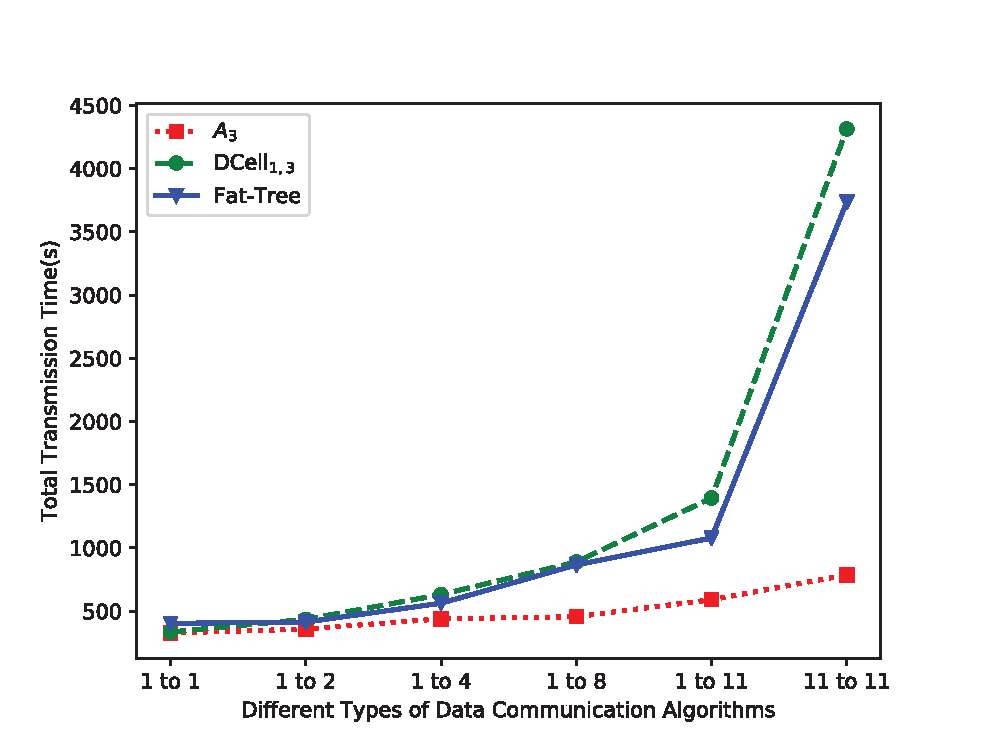
\includegraphics[scale=0.4]{broadcastTime.eps}}
\subfigure[The  average CPU usage rate]{
\label{Fig.sub.2}
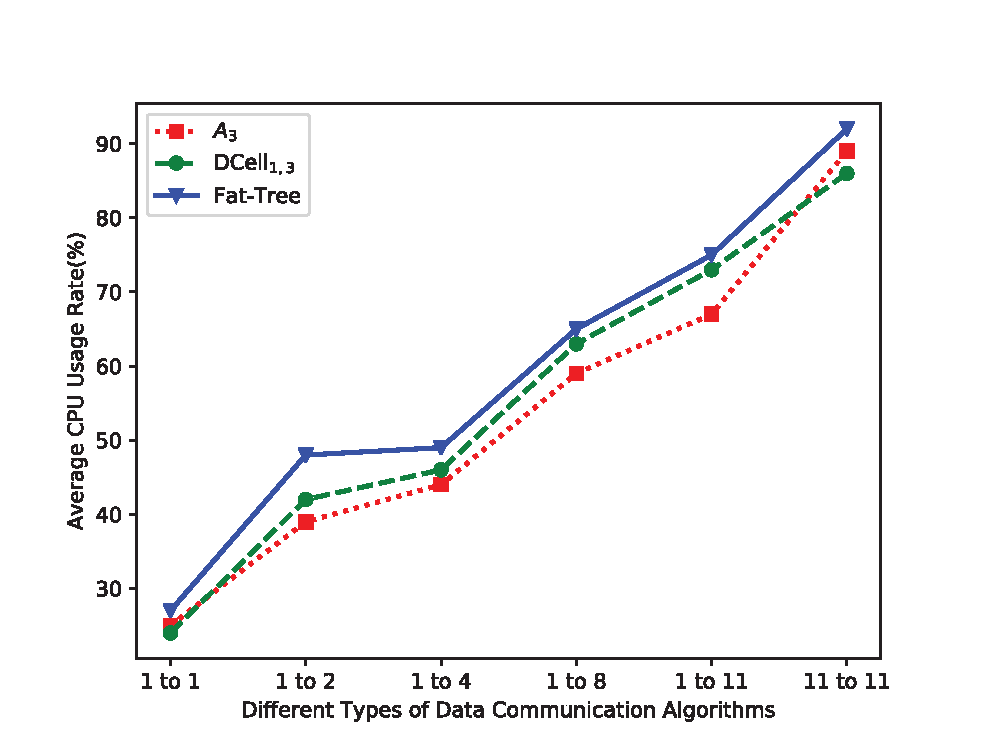
\includegraphics[scale=0.4]{broadcastCpu.eps}}
\caption{The total transmission time and average CPU usage rate of $A_3$, DCell$_{1,3}$, and Fat-Tree in data communication}
\label{broadcast}
\end{figure}

As can be seen from Fig. \ref{Fig.sub.1}, from the perspective of total transmission time, $A_3$ outperforms DCell$_{1,3}$ and Fat-Tree in data communication performance. Especially for one-on-eight,  one-on-eleven, and all to all, the total transmission time of DCell$_{1,3}$ and Fat-Tree is twice or more than the total transmission time of $A_3$. On the other hand, we can see from Fig. \ref{Fig.sub.2} that the average CPU usage rate of $A_3$, DCell$_{1,3}$, and Fat-Tree is almost the same. For example, in the case of all-to-all communication with the highest CPU usage rate, the average CPU usage rates of $A_3$, DCell$_{1,3}$, and Fat-Tree are $89\%$, $86\%$, and $92\%$, respectively. Therefore, it can still be considered that $A_3$ has a better routing performance. In summary, $A_3$ is superior to DCell$_{1,3}$ and Fat-tree in data communication performance.

\subsection{Fault Tolerance of $A_3$, DCell$_{1,3}$, and Fat-Tree}
In this section, we will experiment with fault-tolerant routing for $A_3$, DCell$_{1,3}$, and Fat-Tree, including server fault tolerance, switch fault tolerance, link fault tolerance, and hybrid fault tolerance.
In the fault tolerant experiment of $A_3$ and DCell$_{1,3}$, the number of faulty servers, faulty switches, faulty links  and the number of faulty servers, faulty switches, links in hybrid fault tolerance are 3, 1, 1, (1, 1, 1) and 2, 1, 1, (1, 1, 1). Because the scale of the Fat-Tree we build is small, we do not distinguish the switches in the core layer, aggregation layer and edge layer in the actual fat tree structure of 12 servers, that is, the switches in the core layer, aggregation layer, and edge layer are TL-SG1008PEs. In addition, because the servers in the Fat-Tree are directly connected to the switches in the edge layer, and the connectivity of the Fat-Tree is 1, we will not carry out fault-tolerant experiments on servers failure like BCDC and DCell. Therefore, In the fault tolerant experiment of Fat-Tree, the number of faulty switches, faulty links  and the number of faulty switches, links in hybrid fault tolerance are 1, 1, (1, 1), respectively. We intend to send 5G data from one source server to another destination server and measure the data transfer rate per second and the average CPU usage rate of the server to evaluate the communication performance of these three data center networks. Our fault-tolerant algorithms in BCDC, DCell, and Fat-Tree experiments refer to \ref{restrictedConnectivity}, \cite{GuoC2008}, and \cite{AlFaresM2008}, respectively. In the experiment, we deploy the transmission program on one of the 12 servers in each data center network, and deploy the receiver program on another server, and collect the experimental results after data communication. The experimental results are shown in Fig \ref{faultTolerance}.


\begin{figure}[!h]
\centering
\subfigure[The data transfer rate per second]{
\label{Fig.subft.1}
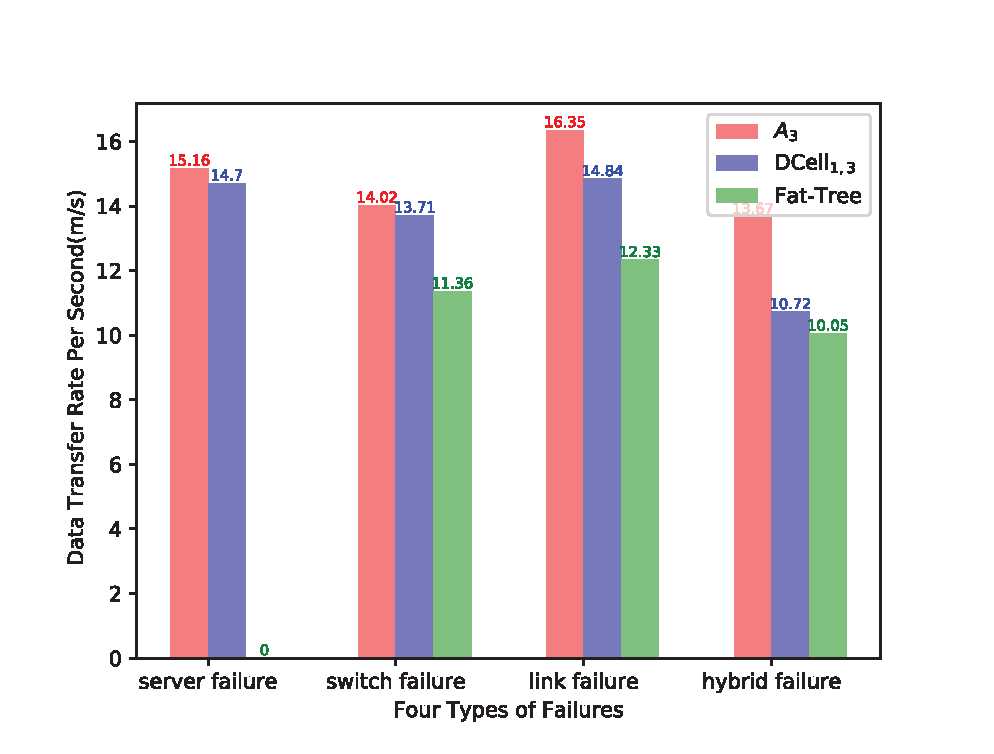
\includegraphics[scale=0.4]{faultToleranceTransferRate.eps}}
\subfigure[The  average CPU usage rate]{
\label{Fig.subft.2}
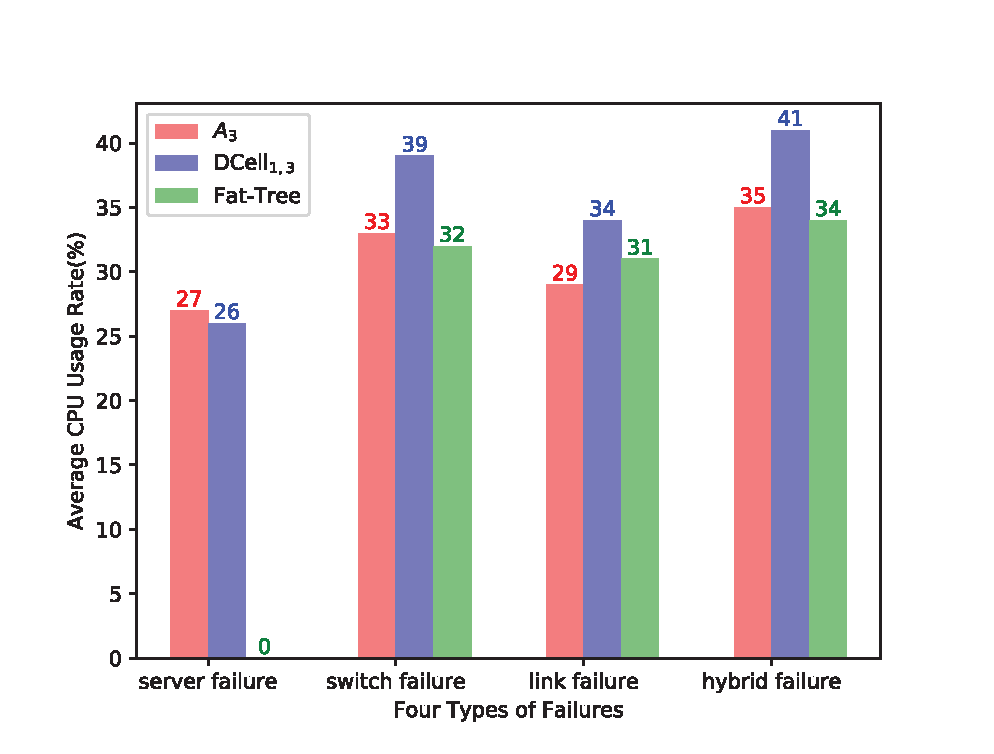
\includegraphics[scale=0.4]{faultToleranceCpu.eps}}
\caption{The data transfer rate per second and average CPU usage rate of $A_3$, DCell$_{1,3}$, and Fat-Tree in fault tolerance}
\label{faultTolerance}
\end{figure}


Since the faulty server in Fat-Tree has no effect on the data communication of other fault-free servers, we have not carried out fault-tolerant experiments of fault server in Fat-Tree. Therefore, we use 0 to replace the experimental results of data transfer rate per second and the average CPU usage rate in the fault-tolerant experiments of fault server in Fat-Tree.

As can be seen from Fig. \ref{Fig.subft.1}, $A_3$ has faster data transfer rate for four fault-tolerant types than DCell$_{1,3}$ and Fat-Tree. On the other hand, $A_3$'s performance on average CPU usage rate is comparable to that of DCell$_{1,3}$ and Fat-Tree in Fig. \ref{Fig.subft.2}. But on the whole, the experimental results of these three data center networks are not much different. Even in the most complex hybrid fault tolerance, the data transfer rate per second and the average CPU usage rate of $A_3$, DCell$_{1,3}$, and Fat-Tree are only 13.67m/s, 10.72m/s, 10.05m/s and $35\%, 41\%, 34\%$. This means that $A_3$ is no worse than DCell$_{1,3}$ and Fat-tree in terms of fault tolerance.

\subsection{Node-Disjoint Paths of $A_3$ and DCell$_{1,3}$}
The third experiment will perform node-disjoint paths experiment on $A_3$. The connectivity on $A_3$ is 4. According to Merger's theorem, there are four node-disjoint paths between any two nodes in 3-dimensional $A_3$. We will arbitrarily select two nodes in the $A_3$ in the experiment, and transmit 5G data through the four node-disjoint paths between these two nodes, and record the transmission time and the average CPU usage rate(ACUR). Similarly, we will evaluate the node-disjoint paths performance of $A_3$ through a comparison experiment with DCell$_{1,3}$. The connectivity of DCell$_{1,3}$ is 3, so there are three node-disjoint paths between any two nodes of the DCell. Since the connectivity of Fat-Tree is 1, there is no more than one node-disjoint paths between any two nodes of Fat-Tree, we don't carry out the node-disjoint paths experiment of Fat-Tree. Our node-disjoint paths algorithms in BCDC and DCell experiments refer to \ref{disjointpaths} and  \cite{WangX2016}. In the experiment, we deploy the transmission program on one of the 12 servers in each data center network, and deploy the receiver program on another server, and collect the experimental results after data communication. The experimental results are shown in Table \ref{node-disjoint paths}.

\begin{table}[!h]
\centering
\caption{The transmission time and the average CPU usage rate of node-disjoint paths in $A_3$ and DCell$_{1,3}$}
%\begin{threeparttable}
\begin{tabular}{|c|c|c|c|}
\hline

\multicolumn{1}{|c|}{ \multirow{2}*{Structure} }&
\multicolumn{2}{|c|}{node-disjoint paths}\\
\cline{2-3}
&time&ACUR\\
\cline{1-3}
$A_3$&220s&43\%\\
\cline{1-3}
DCell$_{1,3}$&245s&46\%\\
\hline
\end{tabular}
\label{node-disjoint paths}
\end{table}

It can be seen from Table \ref{node-disjoint paths}, compared with 328s for one-to-one transmission of 5G data between two nodes in Fig. \ref{Fig.sub.1}, it only takes 220s for $A_3$ to transmit 5G data through four node-disjoint paths between two nodes, which significantly improves the transmission efficiency and effectively improves the data bandwidth. Besides, the performance of  node-disjoint paths in $A_3$ and DCell$_{1,3}$ is similar in terms of transmission time and average CPU usage rate, which also shows that the data center network BCDC has good performance in terms of node-disjoint paths.

Through the above three experiments, we can know that $A_3$ has good properties in data communication, fault-tolerant routing and node-disjoint paths. Although the scale of three experiments is not large, it can also reflect that BCDC is a new data center network with great potential.






\section{Conclusion}\label{conclusion}

In this paper, we introduce the data communication, fault
tolerance, and node-disjoint paths algorithms of BCDC and carry out  corresponding experiments, and compare them with other two other data center networks, DCell and Fat-Tree. The experimental results show that BCDC is superior to DCell and Fat-Tree in data communication. Moreover, in terms of fault-tolerant routing and node-disjoint paths, the performance of BCDC is no worse than that of DCell and Fat-Tree. At the same time, we propose the algorithm for one-to-one communication under 1-restricted connectivity, analyze the complexity of the algorithm, and give an upper bound of the conditional faulty diameter of BCDC under 1-restricted connectivity, which reflects the good fault tolerance of BCDC. The work in this paper shows that BCDC is a better data center network.

\section*{Acknowledgment}

This work was supported by the National Natural Science Foundation of China (No. 61572337, No. 61972272, No. 61602333, and No. 61702351), the National Natural Science Foundation of China (No. U1905211), the Natural Science Foundation of the Jiangsu Higher Education Institutions of China (No. 18KJA520009), the Priority Academic Program Development of Jiangsu Higher Education Institutions, and the Natural Science Foundation of the Jiangsu Higher Education Institutions of China under Grant No 17KJB520036.

%\section*{References}

\begin{thebibliography}{00}
%1
\bibitem{Chang2000Edge}
C. P. Chang, T. Y. Sung, and L. H. Hsu, ``Edge congestion and topological properties of crossed cubes,'' IEEE Transactions on Parallel and Distributed Systems, vol. 11, no. 1, pp. 64-80, 2000.

%2
\bibitem{GuoJ2019}
J. Guo, D. Li, and M. Lu, ``The g-good-neighbor conditional diagnosability of the crossed cubes under the PMC and MM* model,'' Theoretical Computer Science, vol. 755, pp. 81-88, 2019.

%3
%\bibitem{WangS2018}
%S. Wang, and X. Ma, ``The g-extra connectivity and diagnosability of crossed cubes,'' Applied Mathematics and Computation, vol. 336, pp. 60-66, 2018.

%4
\bibitem{DBLPEfe}
K. Efe, ``A variation on the hypercube with lower diameter,'' IEEE Transactions on Computers, vol. 40, no. 11, pp. 1312-1316, 1991.

%5
%\bibitem{ChenHC20}
%H. C. Chen, T. L. Kung, L. H. Hsu, ``An augmented pancyclicity problem of crossed cubes,'' The Computer Journal, vol.61, no.1, pp.54-62, 2018.

%6
%\bibitem{EfeK1992}
%K. Efe, ``The crossed cube architecture for parallel computation,'' IEEE Transactions on Parallel and distributed Systems, vol.3, no.5, pp.513-524, 1992.

%7
\bibitem{AlFaresM2008}
M. Al-Fares, A. Loukissas, and A. Vahdat, ``A scalable, commodity data center network architecture,'' ACM SIGCOMM Computer Communication Review, vol. 38, no. 4, pp. 63-74, 2008.

%8
\bibitem{GuoC2009}
C. X. Guo, G. H. Lu, D. Li, H. T. Wu, X. Zhang, Y. F. Shi, et al. ``BCube: a high performance, server-centric network architecture for modular data centers,'' ACM SIGCOMM Computer Communication Review, vol. 39, no. 4, pp. 63-74, 2009.

%9
\bibitem{GuoC2008}
C. Guo, H. Wu, K. Tan, L. Shi, Y. G. Zhang, and S. W. Lu, ``Dcell: a scalable and fault-tolerant network structure for data centers,'' ACM SIGCOMM Computer Communication Review, vol. 38, no. 4, pp. 75-86, 2009.

%10
%\bibitem{Zhengk2016}
%K. Zheng, L. Wang, B. H. Yang, Y. Sun, S. Uhlig, ``Lazyctrl: A scalable hybrid network control plane design for cloud data centers,'' IEEE Transactions on Parallel and Distributed Systems, vol.28, no.1, pp.115-127, 2016.

%11
%\bibitem{BhuyanLN1984}
%L. N. Bhuyan, D. P. Agrawal, ``Generalized hypercube and hyperbus structures for a computer network,'' IEEE Transactions on computers, vol.C-33, no.4, pp.323-333, 1984.

%12
\bibitem{XuM2019}
M. Xu, J. Diakonikolas, E. Modiano, and S. Subramaniam, ``A hierarchical WDM-based scalable data center network architecture,'' arXiv preprint arXiv:1901.06450, 2019.

%13
\bibitem{NasirianS2019}
S. Nasirian, and F. Faghani, ``Crystal: A scalable and fault-tolerant Archimedean-based server-centric cloud data center network architecture,'' Computer Communications, vol. 147, pp. 159-179, 2019.

%14
\bibitem{XieP2019}
P. Xie, H. Gu, K. Wang, X. Yu, and S. Ma, ``Mesh-of-Torus: a new topology for server-centric data center networks,'' The Journal of Supercomputing, vol. 75, no. 1, pp. 255-271, 2019.

%15
\bibitem{LvM2018}
M. Lv, S. Zhou, X. Sun, G. Lian, and J. Liu, ``Reliability evaluation of data center network DCell,'' Parallel Processing Letters, vol. 28, no. 04, 2018.



%16
%\bibitem{MisraS2019}
%S. Misra, A. Mondal, and S. Khajjayam, ``Dynamic big-data broadcast in fat-tree data center networks with mobile IoT devices,'' IEEE Systems Journal, pp. 1-8, 2019.

%17
\bibitem{LeisersonCE1985}
C. E. Leiserson, ``Fat-trees: universal networks for hardware-efficient supercomputing,'' IEEE transactions on Computers, vol. 100, no. 10, pp. 892-901, 1985.

\bibitem{LvMJ}
M. Lv, B. Cheng, J. Fan, X. Wang, J. Zhou, and Y. Wang, ``The conditional reliability evaluation of data center network BCDC,'' unpublished.


%18
\bibitem{wang2018bcdc}
X. Wang, J. X. Fan, C.-K. Lin, and J. Y. Zhou, ``BCDC: a high-performance, server-centric data center network,'' Journal of Computer Science and Technology, vol. 33, no. 2, pp. 400-416, 2018.

%19
\bibitem{WangDisjointPath}
X. Wang, J. Fan, B. Cheng, J. Zhou, and S. Zhang, ``Node-disjoint paths in BCDC networks,'' Theoretical Computer Science, 2019, unpublished.

%20
\bibitem{WangX2016}
X. Wang, J. Fan, C.-K Lin, and X. Jia, ``Vertex-disjoint paths in DCell networks,'' Journal of Parallel and Distributed Computing, vol. 96, pp. 38-44, 2016.

%\bibitem{LiX2018}
%X. Li, J. Fan, C.-K. Lin, and X. Jia, ``Diagnosability evaluation of the data center network DCell,'' The Computer Journal, vol. 61, no. 1, pp. 129-143, 2018.
%
%\bibitem{LiXJ2019}
%X.-J. Li, M. Liu, Z. Yan, and J.-M. Xu, ``On conditional fault tolerance of hierarchical cubic networks,'' Theoretical Computer Science, vol. 761, pp. 1-6, 2019.
%
%\bibitem{LinL2018}
%L. Lin, S.-Y. Hsieh, R. Chen, L. Xu, and C.-W. Lee, ``The relationship between g-restricted connectivity and g-good-neighbor fault-diagnosability of general regular networks,'' IEEE Transactions on Reliability, vol. 67, no. 1, pp. 285-296, 2018.

\end{thebibliography}
\vspace{12pt}
\color{red}

\end{document}
